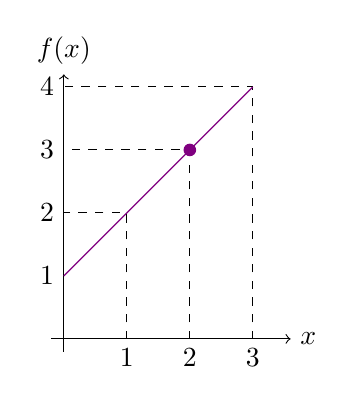
\begin{tikzpicture}[scale=0.8]
    \draw[->] (-0.2,0) -- (3.6,0) node[right] {$x$};
    \draw[->] (0,-0.2) -- (0,4.2) node[above] {$f(x)$};
    %
    \draw[dashed] (0,0) -- (0,1) node[left]{$1$};
    \draw[dashed] (1,0) node[below]{$1$} -- (1,2) -- (0,2) node[left]{$2$};
    \draw[dashed] (2,0) node[below]{$2$} -- (2,3) -- (0,3) node[left]{$3$};
    \draw[dashed] (3,0) node[below]{$3$} -- (3,4) -- (0,4) node[left]{$4$};
    %
    \draw[violet] (0,1) -- (3,4);
    \fill[violet] (2,3) circle[radius=1mm];
\end{tikzpicture}